\documentclass{sigchi}

% Remove or comment out these two lines for final version
\toappearbox{\Large Submitted to CHI'13. \\Do not cite, do not circulate.}
\pagenumbering{arabic}% Arabic page numbers for submission. 

% Use \toappear{...} to override the default ACM copyright statement (e.g. for preprints).

% Load basic packages
\usepackage{balance}  % to better equalize the last page
\usepackage{graphicx} % for EPS, load graphicx instead
\usepackage{times}    % comment if you want LaTeX's default font
\usepackage{url}      % llt: nicely formatted URLs

% llt: Define a global style for URLs, rather that the default one
\makeatletter
\def\url@leostyle{%
  \@ifundefined{selectfont}{\def\UrlFont{\sf}}{\def\UrlFont{\small\bf\ttfamily}}}
\makeatother
\urlstyle{leo}

% To make various LaTeX processors do the right thing with page size.
\def\pprw{8.5in}
\def\pprh{11in}
\special{papersize=\pprw,\pprh}
\setlength{\paperwidth}{\pprw}
\setlength{\paperheight}{\pprh}
\setlength{\pdfpagewidth}{\pprw}
\setlength{\pdfpageheight}{\pprh}

%% Puts space after macros, unless followed by punctuation
\usepackage{xspace}

%%% Personal macros
%% Tired of typing CO2 so many times, requires xspace package
\newcommand{\COtwo}{CO\ensuremath{_2}\xspace}
%% Hawai`i with okina
\newcommand{\Hawaii}{Hawai`i\xspace}
%% Hawai`ian with okina
\newcommand{\Hawaiian}{Hawai`ian\xspace}
%% Manoa with kahako
\newcommand{\Manoa}{M\=anoa\xspace}
%% Formatting W, Wh, kW, kWh properly as units
\newcommand{\W}{\,W\xspace}
\newcommand{\Wh}{\,Wh\xspace}
\newcommand{\kW}{\,kW\xspace}
\newcommand{\kWh}{\,kWh\xspace}

% Make sure hyperref comes last of your loaded packages, 
% to give it a fighting chance of not being over-written, 
% since its job is to redefine many LaTeX commands.
\usepackage[dvips]{hyperref}
\hypersetup{
pdftitle={SIGCHI Conference Proceedings Format},
pdfauthor={LaTeX},
pdfkeywords={SIGCHI, proceedings, archival format},
bookmarksnumbered,
pdfstartview={FitH},
colorlinks,
citecolor=black,
filecolor=black,
linkcolor=black,
urlcolor=black,
breaklinks=true,
}

%% Make links to captions point to the figure, not just the caption at bottom
\usepackage[all]{hypcap}

% create a shortcut to typeset table headings
\newcommand\tabhead[1]{\small\textbf{#1}}

%% Since I'm using the LaTeX Makefile that uses dvips, I need this
%% package to make URLs break nicely
\usepackage{breakurl}

% End of preamble. Here it comes the document.
\begin{document}

\title{The Kukui Cup: A Serious Game About Energy}

% Note that submissions are blind, so author information should be omitted
%\numberofauthors{3}
%\author{
%  \alignauthor Robert S. Brewer, Yongwen Xu, George E. Lee, Michelle Katchuck, Carleton A. Moore, Philip M. Johnson\\
%    \affaddr{Department of Information and Computer Sciences}\\
%    \affaddr{University of Hawaii at Manoa}\\
%    \email{rbrewer@hawaii.edu, yxu@hawaii.edu, gelee@hawaii.edu, johnson@hawaii.edu}\\
%}

% Teaser figure can go here
%\teaser{
%  \centering
%  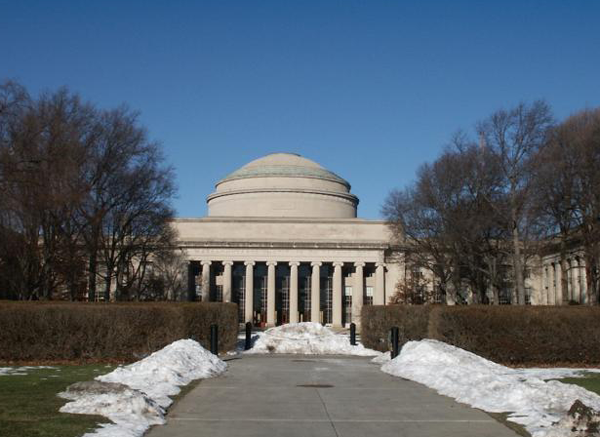
\includegraphics{Figure1}
%  \caption{Teaser Image}
%  \label{fig:teaser}
%}

\maketitle

\begin{abstract}
Insert abstract here.
\end{abstract}

\keywords{
	keyword 1; keyword 2; keyword 3;
}

\category{H.5.m.}{Information Interfaces and Presentation (e.g. HCI)}{Miscellaneous}
%{K.8.0.}{Personal Computing}{Games}

%\\
%\textcolor{red}{See: \url{http://www.acm.org/about/class/1998/}
%for more information and the full list of ACM classifiers and descriptors. 
%Mandatory section: On the submission page
%only the classifiers' letter-number combination will need to be entered.}


\terms{
	Human Factors; Design; Measurement.
}

\section{Introduction}

There has been an ongoing conversation in the HCI community about how we can work to towards the goal of environmental sustainability [cites]. As shown by the surveys by Froehlich et al.~\cite{Froehlich2010} and Pierce and Paulos~\cite{Pierce2012-BEM}, a substantial amount of the research in sustainable HCI has revolved around eco-feedback technology and more specifically around work on electricity consumption feedback. There has also been criticism of the general thrust of this segment of sustainable HCI research. Froehlich et al. point out the lack of communication between HCI researchers and the field of environmental psychology, as well as the relative dearth of long-term field studies in HCI eco-feedback research. Pierce and Paulos point out the general failure of sustainable HCI researchers to address emerging energy systems such as the smart grid and demand response. Brynjarsd\'{o}ttir et al. go further and critique the entire range of recent persuasive sustainability research as focusing overly on optimization of simple metrics and individual action to the detriment of the more complex reality of sustainability~\cite{Brynjarsdottir2012-unpersuaded}.

In this context, we have developed the Kukui Cup Challenge, a serious game~\cite{Zyda2005} designed around topic of energy that incorporates electricity consumption feedback, a multifaceted online game with educational activities, and real-world activities such as workshops and excursions~\cite{csdl2-10-07}. The two primary goals of the Kukui Cup are to teach players how to use less energy, and to improve their \emph{energy literacy} from the level of understanding what a kilowatt-hour is to grasping the major energy policy issues that we confront.

The state of Hawai`i faces a number of unique challenges in the pursuit of sustainability for its citizens, compared to other states. Hawai`i has fertile 
agricultural land, and a variety of renewable energy sources (wind, solar, geothermal, wave), but it imports 85\% of its food, and imports over 90\% of its energy, in the form of oil and coal. In fact, Hawai`i is the most fossil fuel-dependent state in the United States. The Kukui Cup is designed in the context of these challenges, and as an archipelago the issues are felt more keenly than in many other parts of the world.

In this paper we describe the Kukui Cup system, our results from developing and deploying the Kukui Cup in the field, and the lessons learned that we believe would be helpful to other researchers in sustainable HCI. Specifically, we believe that eco-feedback systems should be actionable, that education must go hand in hand with persuasive sustainability systems, and that eco-feedback alone is unlikely to lead to changes in behaviors and attitudes.

\section{The Kukui Cup}

College residence hall energy competitions have become a widespread mechanism for engaging students in energy issues, with more than 160 taking place or being planned for the 2010--2011 academic year~\cite{Hodge2010}. Residence hall energy competitions are events where residence halls or floors within a residence hall compete to see which building will use the least energy over a period of time. Some competitions pull in other aspects of environmental sustainability, including reducing water usage, reduced waste production, etc. The competitions tap into both the residents competitive urges, and their interest in environmental issues. However, unlike a home environment, the residents typically do not financially benefit from any reduction in electricity use resulting from their behavior changes, since residence hall fees are flat-rate and do not change based on energy usage. This leads to residents being completely unaware of their energy usage, since they lack even a monthly bill as feedback. Dillahunt et al. describe similar a similar situation with their investigation of energy usage in low income communities, where individuals may not be billed directly for electricity and may not have the means to upgrade appliances~\cite{Dillahunt2009-low-income}. Despite these differences, Dillahunt et al. found that the residents of low-income housing were still motivated to save energy and came up with diverse energy-saving solutions, which may suggest that dorm residents can be similarly motivated.

Residence hall energy competitions range in complexity from simple web pages updated weekly with electricity data to complicated web applications (\cite{csdl2-11-01}, pg 6--11). Oberlin College was an early adopter of the residence hall energy competition and developed a real-time electricity consumption feedback system as described by Petersen et al.~\cite{petersen-dorm-energy-reduction}

To build on this area of active energy work, we decided to target our serious game to college students living in residence halls. The Kukui Cup extends the college energy competition, which is often focused primarily on reducing electricity use as measured by some metering infrastructure, into a broader energy \emph{challenge} where electricity consumption feedback is only one part of a larger game experience for players. The challenge is named after the kukui nut (also known as candlenut), which was burned by Native Hawaiians to provide light, making it an early form of stored energy in \Hawaii.

In a Kukui Cup challenge, residents are grouped into teams based on where they live. Teams can be different floors of a building or entire buildings. The electricity usage of teams is measured either through manual meter readings or through automated meter data collection. In addition to the energy competition, the Kukui Cup has a point competition where players can earn points by engaging in educational and social activities on the challenge website such as watching short videos about energy as well as attending real-world events. The point system provides a way to motivate players to explore and use the system, as the Kukui Cup is currently intended as an extracurricular activity.

\begin{figure}[!t]
\centering
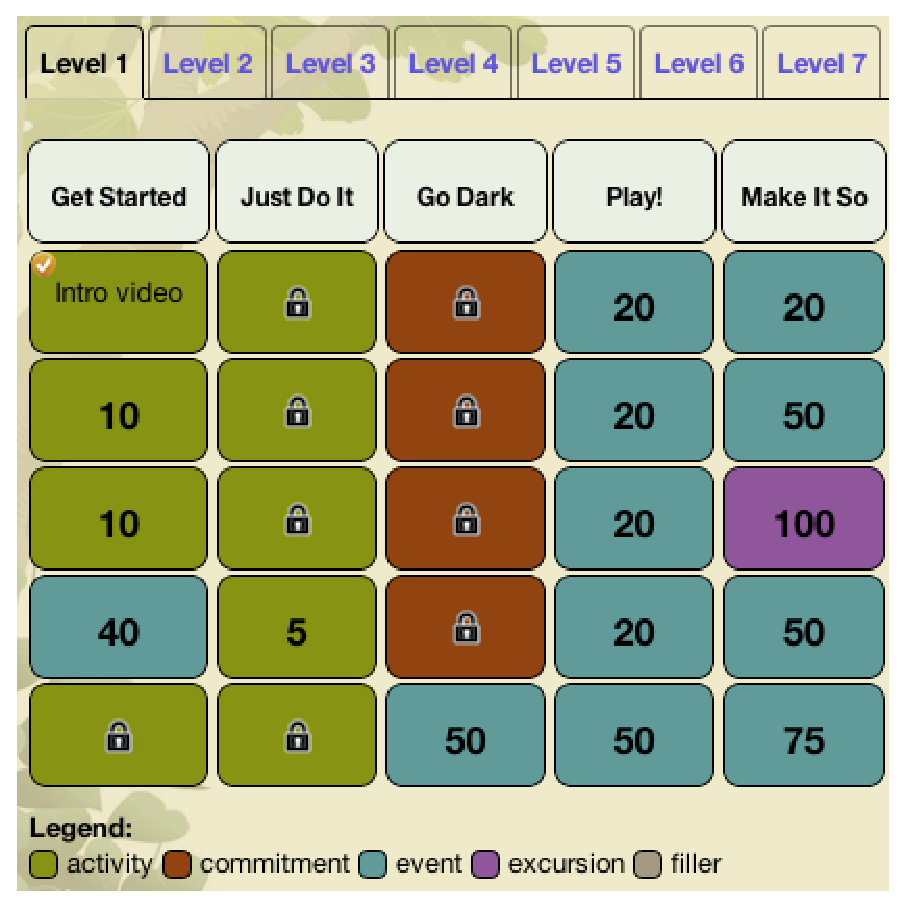
\includegraphics[width=0.95\columnwidth]{smart-grid.eps}
\caption{The Smart Grid Game widget, displaying the actions available in level 1.}
\label{fig:smart-grid}
\end{figure}

Much of the point competition revolves around a section of the challenge website called the Smart Grid Game (SGG). The Smart Grid Game consists of rows of actions arranged into columns based on a particular topic (similar to the popular game show ``Jeopardy''), shown in \autoref{fig:smart-grid}. Clicking on a square in the SGG shows details about the action and explains how players can complete the action to earn points. There are several types of actions: short YouTube videos on energy and sustainability topics, activities like measuring the flow rate of a shower, excursions such as visiting a farm that produces all its own electricity, and commitments such as carpooling or not eating meat. There are also creative actions such as writing a poem about energy or a letter to the editor on a sustainability topic. The flexibility of the SGG allows us to provide a wide variety of interesting actions for players to take part in.

The completion of each action (with the exception of commitments) is verified through the challenge website before points are awarded. For activities, players are usually asked a randomly-selected question, and their answer is placed in a queue for challenge administrators to review. The administrator can approve or reject the submission, and can provide feedback on the answer to the player. The game also supports activities that are verified by submission of an uploaded image such as a photo or screenshot.

Kukui Cup challenges can also choose to provide incentives to players in the form of prizes both at the individual (points) and team level (points and energy use). One problem with the prizes provided in the competition as incentives is that they only go to the top performers in each competition. For those participants that are aware that they will not win the point competitions, the prizes provide little incentive, or possibly a disincentive: why play if there is no way to win a prize? Another problem with the prizes is that to be effective they had to appeal to all participants, limiting the options for prizes.

We developed the Raffle Game to provide a prize-based incentive to play that was not limited to the top players, through inspiration from Prabhakar's work incentivizing road congestion reduction~\cite{Merugu2009}. In the Raffle Game, there are a variety of raffle prizes available in each round of the competition. For each 25 points a participant earns, they receive a virtual raffle ticket. Participants can allocate their raffle tickets among the prizes available, and they can change their allocations at any time. At the end of the round, the raffle is closed and the ticket allocations frozen. A winning ticket is ``drawn'' from those allocated to each raffle prize, and the owner of that ticket wins the prize.

\subsection{Running a Kukui Cup}

A Kukui Cup challenge consists of multiple components working together to provide the entire game experience. For challenges using real-time energy data, open source WattDepot~\cite{csdl2-10-05} system is used to collect, store, and analyze the data. The challenge website and associated game mechanics are provided by the open source Makahiki system~\cite{csdl2-11-07}. Educational content is tailored to the needs of college students living in residence halls in \Hawaii, but still needs to be customized for each institution hosting the challenge.

The final component in a Kukui Cup challenge are the administrators. Challenge administrators need to plan out the parameters of the competition (length, number of teams), make game design choices such as point rubrics, customize the educational content for their organization, organize workshops, review player verification submissions, and distribute prizes. Kukui Cup challenges are labor intensive, but that labor provides the opportunity to interact with the players more fully and provide them with a expansive game experience.

\subsection{Field Evaluations}

In addition to in-lab evaluations and beta tests, there have been two sets of field evaluations of Kukui Cup challenges. The first Kukui Cup challenge took place over 3 weeks starting in October 2011 in four residence halls for first-year students on the University of \Hawaii at \Manoa campus containing a total of approximately 1070 residents. Each residence hall was further broken into five pairs of floors, each of which share a common lounge area. These pairs of floors are referred to as \emph{lounges}, and were the team unit in the 2011 Kukui Cup.

The second set of challenges is taking place starting in September 2012. The University of \Hawaii (UH) Kukui Cup is taking place in the same four residence halls with approximately the same number of residents. However, instead of three weeks, the 2012 UH Kukui Cup will take place over the entire nine month academic year. The first month of the competition will be an intensive period with multiple real-world events taking place each week, while the remaining months will be less intensive. The goal of the much longer time frame is to discourage short-term and unsustainable behaviors (such as forgoing all electronic device use). 

In addition to the 2012 UH Kukui Cup, Hawaii Pacific University (approximately 200 residents) and the East-West Center (approximately 130 residents) are both running their own challenges using the Kukui Cup system with our support.

\section{Baselines and Goals}
\label{sec:goals-baselines}

Goals have been shown to be effective tools in changing energy consumption behavior~\cite{Becker78, Houwelingen89}. Setting achievable goals is important from a gameplay perspective, so goals must typically be based on previous energy use. The most common way to generate a goal is to calculate a \emph{baseline} of energy usage based on past energy usage, and then set the goal as some percentage reduction from the baseline.

Two of the most common ways to calculate the electricity baseline are to average recent prior usage (such as the last two weeks), or to average usage from previous years. Both of these methods are problematic because they assume that this previous usage is representative of future usage, even though there are many factors that can significantly alter electricity use over time including: occupancy, weather, activities (e.x., studying for a big midterm exam), and changes to the building infrastructure such as efficiency upgrades. Any of these factors can lead to the baseline being an inaccurate predictor of future usage in an energy competition, as described by Johnson et al.~\cite{csdl2-12-08}.

Since baselines can be poor predictors of future electricity use, comparing actual electricity use to the baseline in order to determine how much electricity was ``saved'' by an intervention is misleading and can tempt designers to make claims about energy saved that cannot be substantiated. However, comparison of actual electricity usage to a goal generated from a baseline can be helpful as a game mechanic to motivate players to conserve energy.

In the 2011 Kukui Cup, we used a baseline that was derived from an average of the two weeks prior to the challenge. In the 2012 Kukui Cups, we have switched to a dynamic baseline~\cite{csdl2-12-08} that consists of the average electricity usage for the two previous weeks, but the baseline is recomputed every day throughout the challenge. This means that as the challenge progresses, the baseline will include usage during the challenge. In essence, a goal generated from a dynamic baseline requires a team to reduce their energy usage compared to the recent past. Since the baseline is not a static value picked once before the challenge, anomalous conditions during the period before the challenge will soon be replaced with new, more representative data.

We incorporate the energy goal into a game called the Daily Energy Goal Game (DEGG). Each team has a daily energy goal determined by the baseline. When a team's energy usage at the end of the day is equal to or below the goal, they win the DEGG for that day. In the 2012 Kukui Cups, the energy competition is scored by the number of daily energy goals that each team has achieved, rather than an absolute measure of how much energy has been used or how much a team has reduced their usage below the baseline. By counting goals rather than measures of absolute or relative energy reductions, we hope to incentivize sustainable longer-term behavior changes rather than radical short-term changes such as moving out of the residence hall and into tents (as has been reported anecdotally in some other energy competitions). In an effort to link the energy and point competitions, when a team meets their daily energy goal, each team member receives a configurable number of points.


\section{Electricity Feedback in the Kukui Cup}

Feedback on electricity consumption has been used as a means for facilitating energy conservation both in the CHI community~\cite{Froehlich2010} and the broader energy efficiency~\cite{darby-review-2006, Faruqui09, Foster-2012} and environmental psychology~\cite{Becker78, Houwelingen89} communities. One reason for this focus on feedback is undoubtedly the hidden nature of electricity, so feedback provides an awareness that is otherwise unavailable.

One of the fundamental principles of energy visualizations and feedback displays in the Kukui Cup is that they be \emph{actionable}. We feel strongly that eco-visualizations that do not guide viewers towards actions they can take will be ineffective in changing viewers energy use behaviors. While any energy feedback visualization may implicitly encourage energy conservation behaviors simply by making energy use visible, this does not meet our definition of actionable. A feedback display that shows that a home has used 20 kWh so far on a particular day leaves the viewer with natural questions: is that a lot? what should I do if I wanted to reduce my energy use?

\begin{figure}[!t]
\centering
\includegraphics[width=0.7\columnwidth]{energy-24hours-new.eps}
\caption{A bar chart visualization of energy use as compared to a goal over 24 hours}
\label{fig:energy-24hours}
\end{figure}

\subsection{Initial Visualization}
Our first attempt at electricity visualizations for the Kukui Cup are shown in~\autoref{fig:energy-24hours}. The bar graph shows hourly energy use for a pair of floors participating in the Kukui Cup over 24 hours as compared to an energy goal. Note that the data shown in this particular figure is simulated. Bars that are entirely green show the actual energy usage for that hour and indicate that the energy use was below the hourly goal. For mixed red and green bars, the green portion represents the energy goal for that hour of the day, while the red portions represent the actual usage in excess of the goal.

The bar graph visualization shows the variation of energy use over the course of a day, which is an important energy literacy concept. It also shows what parts of the day energy use is exceeding the goal, and by how much. By displaying the times during the day when the hourly goals are not being met, residents could focus on understanding what activities are going on during those periods.

After presenting this bar chart visualization to colleagues and friends, there was a strong sentiment that the visualization was too complicated to be understood effectively by participants in the context of the Kukui Cup. We therefore abandoned the bar chart in favor of even simpler visualizations.

\subsection{Simplified Visualizations}
\label{sec:simple-viz}

\begin{figure}[!t]
\centering
\includegraphics[width=0.95\columnwidth]{degg.eps}
\caption{The Daily Energy Goal Game visualization}
\label{fig:degg}
\end{figure}

To make the visualization easier to understand and also more actionable, we developed the Daily Energy Goal Game (DEGG) visualization shown in~\autoref{fig:degg}. The most prominent parts of the DEGG are: the energy consumption so far during the current day, the energy goal so far for the current day, and a traffic light that shows in the most straightforward way whether the team is meeting their energy goal. The display updates once every 10 minutes with new energy data.

We picked the daily time frame for the game for two reasons. First, having a daily goal makes behavior changes more visible and feedback more immediate than a longer time frame such as weekly or monthly. Second, by concentrating on a daily goal, teams that are performing poorly on a particular day can redouble their efforts by doing better the next day. Similarly, a team that does particularly well for one day cannot rest on their laurels, they must make an effort to conserve on every day. This reflects our belief that changing energy behaviors is a marathon and not a sprint: radical short-term changes made to win an energy competition are unlikely to be sustainable, and are therefore of very limited utility.

Residential energy use varies in intensity over the course of a day: typically low when people are sleeping and much higher during evening hours. For the students in the residence halls in our studies, the energy usage peak occurs at approximately midnight, and the lowest value is between 8 and 9 AM, which is considerably different than an average single-family home. There is also daily variation between days of the week, as the activities taking place on a Monday night are different than those on a Saturday night. To account for the hourly and daily variation in energy use, our we compute hourly and daily baselines for energy use, and the goal value is a percentage reduction from the baseline. The energy consumption and goal values displayed in the DEGG are computed over the time period from midnight to the current time. This is particularly important for the goal value, because if a daily goal value was simply spread linearly over the course of a day, players would see their energy use as always under the goal during low-usage periods, but then going above the goal during the high-usage periods, possibly to a degree that makes it impossible to meet the goal for that day.

Below the traffic light display of the DEGG is a list of actions from the Smart Grid Game that players can take to either learn more about energy, or directly help reduce their energy use. The actions displayed depend on what actions the player has already completed in the rest of the system. The direct links to actions that players can take to reduce their energy usage, tailored to the opportunities available in their residence hall make the DEGG highly actionable.

In another attempt to make visualizations actionable, we created a small widget below the DEGG titled ``How can we make our daily goal?''. This widget, shown in~\autoref{fig:make-goal}, showed how much the player's team energy usage was above the goal, and provided a drop-down menu of electrical devices commonly present in student rooms: laptops, XBox 360, Wii, etc. When a device was selected from the menu, the system would display the approximate number of hours of device use that would equal to the amount of team energy use over the goal value. The time value was intended to show players how much device use they would need to \emph{forego} in order to get back on track to their energy goal, and develop their intuition about the relative power use of different devices (i.e., plasma TVs use much more power that Wii game consoles). Therefore a short time value could point out an easy way to make the goal, and a long time value would indicate less significant energy conservation.

However, during in-lab evaluations of the system, we found that multiple subjects misinterpreted the time value, thinking that high time values were bad rather than good. Since the Wii was the device on the list with the smallest power use (20 W), it led to the highest time values. Some subjects drew the conclusion that using a Wii was worse than using an XBox 360 or Playstation 3, which was precisely the opposite goal of this widget. One subject even took the time to use our in-game team discussion forum to post the message ``don't play wii'' after using the widget! Because of this example, we dubbed this confusion the ``Wii problem''.

We were ultimately unable to come up with a way to display this information in a way that would be both actionable, and not confusing to players. Given the risk of players mistakenly drawing the opposite conclusions that we intended, we ended up removing this widget from the system before it was put into production. The ``Wii problem'' demonstrates the challenges in making energy feedback actionable with a user population that is generally energy illiterate.

\begin{figure}[!t]
\centering

\includegraphics[width=0.6\columnwidth]{how-meet-goal.eps}
\caption{The ``How can we make our daily goal?'' widget}
\label{fig:make-goal}
\end{figure}


\subsection{The Canopy}

The 2011 Kukui Cup took place over three weeks, and as part of the game experience we wanted to provide another level of experience for the top participants in the competition. The background of the competition website featured a forest theme, so the Canopy was named to convey that it existed ``above'' the rest of the website. The Canopy was conceived as a way to keep the top participants engaged even if they had completed most of the activities available in the Smart Grid Game.

The Canopy provided a series of ``missions'' that players could undertake. Some Canopy missions were to be accomplished individually, while other missions required 2 or 3 participants to work together. Players could indicate that they were ``up'' for a group mission to find other interested participants. Missions included looking at more advanced energy visualizations, and also activities such as seeking out places on campus that are wasting energy.

Canopy missions were like forest activities, but instead of earning points upon completion, Canopy activities earned \emph{Canopy Karma}, which was a separate point system for the Canopy. Canopy Karma was used instead of the standard points to ensure that the Canopy itself did not unbalance the point competition by providing a way for the top players to earn more points that were not available to the rest of the participants.

The energy data and visualizations described previously were deliberately simple to avoid confusing participants, based on the results of our usability testing. In addition, the energy data shown to players come only from the participant's team. Since the Canopy was intended for the top participants of the competition, who were believed to be more receptive to detailed energy data and data for other lounges, energy visualizations featured prominently in the Canopy. Several of the Canopy missions involved looking at the advanced visualizations and answering questions based on their understanding of the data.

\begin{figure}[!t]
\centering
\includegraphics[width=0.95\columnwidth]{hot-spots-crop.eps}
\caption{The Hot Spots visualization of weekly energy use for a particular team}
\label{fig:hot-spots}
\end{figure}

\autoref{fig:hot-spots} shows the Hot Spots visualization of electricity use for one particular team. The Hot Spot visualization shows hourly electricity use for one team over the course of a week. This allows players to examine their usage patterns and see how they change throughout the day, and how the patterns differ between days of the week. The Canopy mission based around the Hot Spots visualization asked players the following questions:

\begin{itemize}
	\item What hours of the day seem to have the highest energy use? How does that compare to your own energy use patterns?
	\item What differences in energy use do you notice between teams?
	\item What are your thoughts on this visualization? What are its strengths and weaknesses?
\end{itemize}

The Canopy was introduced in the third week of the 2011 Kukui Cup, and the top 42 players were invited to enter the Canopy out of a total of 401 players. Canopy players spent an average of 10 minutes in the Canopy, a small portion of their overall time spent in the Kukui Cup game website. Despite their limited use, players' feedback about the more advanced visualizations was positive: they reported enjoying the ability to compare energy use between teams and seeing what times different teams energy use peaked. Overall, the Canopy did not live up to our expectations as a way for the top players to expand their horizons beyond the central ``forest'' part of the game. We believe the two primary factors to the low usage of the Canopy were: the inability to earn points in the Canopy (instead earning Canopy Karma), and the relatively short period of time the Canopy was available to the players. Based on our experiences from the 2011 Kukui Cup, we have incorporated the visualizations into the later rounds of the much longer 2012 Kukui Cup, which will give players more time to explore and the opportunity to earn normal points.


\section{Energy Literacy}
\label{sec:energy-literacy}

\emph{Energy literacy} is the understanding of energy concepts as they relate both on the individual level and on the national/global level. Solving the world energy crisis will require everyone to understand how energy is generated and consumed, so that they can make more informed choices in their lives and as informed citizens involved in their communities. Energy literacy is also needed at the individual level, since decisions about how conserve energy require an understanding of how energy is used and what actions are most helpful for conservation.

Some examples of energy literacy are:

\begin{itemize}
	\item Understanding the difference between power and energy.
	\item Knowing that a microwave uses much more power than a refrigerator, but that the refrigerator will use much more energy over time.
	\item Knowing how electricity is generated in one's community.
\end{itemize}

There is a proposed renewable energy project in Hawaii called ``Big Wind'' that would generate as much as 400\,MW from wind farms covering substantial portions of two more rural islands (Moloka`i and L\=ana`i) with excellent wind resources. The power would be transmitted via a new undersea cable to O`ahu, which has the majority of the state's population, but inferior wind resources. There are advocates both for and against Big Wind, but to make an informed decision one should understand how O`ahu's electricity is generated now, and the characteristics and challenges of wind energy.

Unfortunately, all indications are that energy literacy is low in the USA. 
DeWaters and Powers have developed an energy literacy survey instrument for middle and high school students~\cite{DeWaters2007,DeWaters2008}. They found that the student mean attitude scores were 73\%, but that knowledge scores lagged far behind (42\% correct)~\cite{DeWaters2011}. Based on their findings, they make some recommendations, including: energy curricula be ``hands on, inquiry based, experiential, engaging, and real-world problem solving \ldots'', and using the campus as a ``learning laboratory''. Similarly a nationwide survey of adults on energy by Southwell et al. found that the average respondent answered fewer than 60\% of the energy knowledge questions correctly~\cite{Southwell2012}.

One energy literacy topic that we emphasize in the Kukui Cup is the difference between power and energy, power being the rate at which energy is being consumed or produced (measured in watts) and energy is the quantity of work that can be performed by a system (measured somewhat confusingly for electricity in kilowatt-hours). In the Kukui Cup we explain this relationship as being analogous to speedometer and odometer in a car.

Through answers submitted to the online activities in the Kukui Cup, we can see that many players have trouble understanding the concepts of power, energy and their interrelationship. Players often confuse the two concepts and often fail to grasp the time sensitivity of power, and thereby considering devices that consume a lot of power as ``bad'' irrespective of how long they are actually used. When the users of visualizations, such as we described earlier, do not understand the concepts that are being visualized, understanding of the visualizations becomes much more difficult. It is for this reason that we claim that eco-feedback systems should incorporate educational components, or risk being unintelligible to users. However, we reject the notion that power and energy, watts and kilowatt-hours are too complicated and that users should be provided instead with analogies to cars driven or hamburgers eaten. These energy concepts are important for our energy future, and should not be hidden from users.

% Short answer questions can prompt players to reflect on their experiences

In addition to shorter activities available in the SGG, the Kukui Cup also provides creative activities to encourage more in-depth explorations of energy and sustainability. These creative activities run the gamut from writing a haiku about a sustainability topic, to conducting an interview, or making a video. Creative activity submissions from players are assigned a point value by administrators based on the quality of the work and the effort required to make. We hope that the creative activities provide a different outlet for players, and encourage them to think beyond their individual actions, as many of the other activities focus on.

As mentioned previously, the 2012 UH Kukui Cup will run for an entire academic year. Much of the educational content we have developed will be made available to players in the first intensive month of the challenge, leaving later rounds with less content, and thereby fewer reasons to continue playing. To address this problem, and to draw players into deeper play and understanding of sustainability issues, players will be able to suggest new additions to the SGG as part of the game. Players that provide useful new activities and events for the the game will earn points, and once the new actions are placed into the SGG, they will have provided additional educational content to their fellow players. We are also exploring ways to tie class work into the Kukui Cup challenge. With the longer time frame afforded by the nine month competition, we intend to allow players to earn points in the competition by registering for sustainability-related classes, and picking sustainability-themed class projects. Ultimately, we hope the Kukui Cup will lead to macro behavior changes like selecting a sustainability degree program or choosing a more efficient vehicle.

We have also witnessed improvements in players' energy literacy in the course of a single workshop. In the energy scavenger hunt workshop, attendees are grouped into teams of 3--4 people and provided with a plug load meter that shows the amount of electrical power consumed by whatever device is plugged into the meter. Each team is given 30 minutes record the power use of devices in their rooms and residence halls, looking for devices with the highest power use they can find, and also the most number of devices with distinct power use in 10\,W intervals. The goals of the workshop (beyond entertainment) are to give players experience measuring device power use, and also to build their intuition about how much power different devices use. In the 2011 Kukui Cup, when the teams gathered together after the 30 minutes was up, each team was asked to present the results of their hunt. One team reported that the microwave they measured used 200\,W, and immediately several players from other teams shouted out that the first team must have done something wrong because microwaves use over 1000\,W, a fact they most likely learned during their own hunt.

As one means of assessing the impact of the 2011 Kukui Cup, we developed an energy literacy questionnaire, based in part on the DeWaters and Powers instrument~\cite{DeWaters2011}. However, \Hawaii's energy situation differs significantly from the US mainland, so we did not use the energy knowledge section of the DeWaters and Powers instrument. For example, in most parts of the US, home heating is the largest consumer of household energy, while in \Hawaii for some homes (especially those that do not use air conditioning) hot water is the largest consumer of household energy.

The energy literacy questionnaire was sent via email to a random sample of residents in the four residence halls both before and after the challenge. 48 subjects completed both the pre and post questionnaires. To distinguish between residents that participated in the Kukui Cup, we classified subjects as participants if they had earned 25 points in the the competition. Players could earn 25 points in several ways, but the simplest way is by logging into the challenge website, watching an introductory video about the challenge, and answering a question about the video correctly. Therefore 25 points represents a conservative threshold for participation, since it could be achieved with a single, short visit the challenge website.

The energy knowledge section of the questionnaire consisted of 19 factual questions about energy, with a specific emphasis on \Hawaii energy issues. \autoref{tab:knowledge-descriptives} shows the average number of questions answered correctly for participants and non-participants in the pre and post-competition questionnaires. Non-participants showed a tiny reduction in questions answered correctly after the competition, while participants improved by 18.8\%.

\begin{table}[htbp]
	\centering
	\small
		\begin{tabular}{ l | c | c | c | c | c }
			\cline{2-5}
			& \multicolumn{2}{c |}{Pre-competition} & \multicolumn{2}{c|}{Post-competition} & \\ \hline
			\multicolumn{1}{|l|}{Subject type} & Mean & Std. Dev & Mean & Std. Dev & \multicolumn{1}{c|}{\% Change} \tabularnewline \hline \hline
			\multicolumn{1}{|l|}{Non-participants} & 7.46 & 2.377 & 7.37 & 2.570 & \multicolumn{1}{c|}{-1.2\%} \tabularnewline \hline
			\multicolumn{1}{|l|}{Participants} & 7.54 & 1.837 & 8.96 & 3.290 & \multicolumn{1}{c|}{18.8\%} \tabularnewline \hline
		\end{tabular}
	\normalsize
	\caption[Energy knowledge before and after competition]{Average number of energy knowledge questions correct for participants and non-participants before and after the competition}
\label{tab:knowledge-descriptives}
\end{table}

Using ANOVA, there was a significant interaction between participation and differences between pre and post-competition scores, F (1, 46) = 3.84, p = 0.056, MSE = 3.52. While the improvement for participants over non-participants was small, it supports the hypothesis that participating in the Kukui Cup improves the energy literacy of participants.


\section{Serious Game vs Eco-Feedback}

There are indications that the long-term impact of eco-feedback may be diminished due to habituation. Froehlich suggests that the average user will spend less than one minute per day exploring their energy consumption behaviors~\cite{Froehlich2010-BECC}. People habituate to feedback [citations?]

Serious games like the Kukui Cup provide an alternative route to promote both learning and engagement with energy feedback. For this reason the Kukui Cup is a serious game that incorporates electricity consumption feedback as one aspect of the game experience, rather than an eco-feedback system that has been gamified. One problem with the serious game approach in the Kukui Cup is that the educational content is largely of interest only once. We do not anticipate that players would want to revisit most actions unless they were able to earn additional points. This is in contrast to most normal games that are notable in how much players enjoy playing them over and over. Some serious games such as the protein folding game Foldit do manage to attract repeat players and meet their serious goals~\cite{Khatib2011}. While the Kukui Cup may stop being of interest to players once they have completed all the content available, we hope that our attempts to engage players in broader sustainability opportunities such as taking classes and becoming involved in campus and community organizations make the Kukui Cup no longer necessary for them.

While games are not the only way to promote long-term engagement with energy issues, we submit that any normal eco-feedback system will quickly be abandoned by users once the novelty wears off. There must be a continuing reason for users to revisit the system that even the finest eco-feedback systems lack.


\section{Conclusion}

Conclusion to go here.

\section{Acknowledgments}

Omitted from review version.

%\textbf{Don't forget
%to acknowledge funding sources as well}, so you don't wind up
%having to correct it later.

% Balancing columns in a ref list is a bit of a pain because you
% either use a hack like flushend or balance, or manually insert
% a column break.  http://www.tex.ac.uk/cgi-bin/texfaq2html?label=balance
% multicols doesn't work because we're already in two-column mode,
% and flushend isn't awesome, so I choose balance.  See this
% for more info: http://cs.brown.edu/system/software/latex/doc/balance.pdf
%
% Note that in a perfect world balance wants to be in the first
% column of the last page.
%
% If balance doesn't work for you, you can remove that and
% hard-code a column break into the bbl file right before you
% submit:
%
% http://stackoverflow.com/questions/2149854/how-to-manually-equalize-columns-
% in-an-ieee-paper-if-using-bibtex
%
% Or, just remove \balance and give up on balancing the last page.
%
\balance

% If you want to use smaller typesetting for the reference list,
% uncomment the following line:
% \small
\bibliographystyle{acm-sigchi}
\bibliography{sustainability,csdl-trs,gamification}
\end{document}
